\documentclass[aspectratio=169]{beamer}
\usetheme{Frankfurt}

\setbeamertemplate{caption}[numbered]
\setbeamertemplate{itemize items}[circle]

\usepackage[ngerman]{babel}
\usepackage{csquotes}
\usepackage[sorting=none,style=numeric]{biblatex}
\usepackage{circuitikz}
\usepackage{siunitx}
\usepackage{pifont}
\usepackage[normalem]{ulem}
\usepackage{svg}

\addbibresource{./sources/spule.bib}
\addbibresource{./sources/images.bib}

\AtBeginBibliography{\small}

\graphicspath{ {./assets/} }

\title{Spulen}
\subtitle{Bedeutung und Wirkung der Induktion}
\author{
    Jana Schnopp \and
    Julien Deutscher \and
    Cornelia Baumbach \and
    Linus Ziegler
}

\institute{Ferdinand-Braun-Schule Fulda}

%% create a title slide for every new section
\AtBeginSection[] {
    \begin{frame}
        \vfill
        \centering
        \begin{beamercolorbox}[sep=8pt, center, shadow=true,rounded=true]{title}
            \usebeamerfont{title}\insertsectionhead\par%
        \end{beamercolorbox}
        \vspace{1cm}
    \end{frame}
}


%% create a title and subtitle for the frame
\def\makeframetitle {
    \frametitle{\insertsubsectionhead}
    \framesubtitle{\insertsectionhead}
}

\begin{document}

\begin{frame}
    \maketitle
\end{frame}

\begin{frame}
    \section*{Inhalt}
    \frametitle{Inhalt}
    \tableofcontents
\end{frame}

\graphicspath{{./assets/}}

\section{Spule}
\subsection{Definition und Aufbau der Spule}
\begin{frame}
    \makeframetitle

    \begin{columns}
        \begin{column}{0.5\textwidth}
            \begin{itemize}
                \item Spiralförmig gewickelter Draht
                \item Passives Bauelemente
                \item \alert{Besondere Eigenschaft}: hohe \textit{Induktivität}
            \end{itemize}
        \end{column}
        \begin{column}{0.5\textwidth}
            \begin{figure}
                \centering
                % \includegraphics[width=0.8\textwidth]{Electronic_component_inductors}
                % \caption{Bild einiger Spulen/Drosseln\cite{miguel_spule_2007}}
            \end{figure}
        \end{column}
    \end{columns}
        
\end{frame}

\begin{frame}
    \makeframetitle
    \begin{itemize}
        \item Meist um einen festen Körper gewickelt
        \item Die einzelnen Windungen müssen voneinander \textit{isoliert}
            sein
        \item Man spricht von einer \alert{Luftspule}, wenn der Wickelkörper
            \textit{nichtmagnetisch} ist
        \item Schaltzeichen der Spule: \\
            \begin{figure}
                \centering
                \begin{circuitikz}
                    \draw
                    (0, 2) to [american inductor, o-o] (0, 0)
                    ;
                \end{circuitikz}
                \caption{Schaltzeichen}
            \end{figure}
    \end{itemize}
\end{frame}

\section{Induktion und Induktivität}
\subsection{Begriff der \textit{Elektromagnetischen Induktion}}
\begin{frame}
    \makeframetitle

    \begin{columns}
        \begin{column}{0.65\textwidth}
            \begin{itemize}
                \item \alert{Wechselwirkung} zwischen
                    \textit{Magnetimus} und \textit{Elektrizität}
                \item Voraussetzung ist ein sich ständig \alert{änderndes}
                    Magnetfeld
                \item Die Induktionsspannung $U_i$ ist messbar, wenn\dots
                    \begin{enumerate}
                        \item ...sich die magnetische Flussdichte \alert{verändert},
                        \item ...der Flächeninhalt der Leiterschleife
                            sich \alert{verändert}
                        \item ...sich die Weite des Winkels
                            zwischen magnetischem Feld und der Leiterschleife
                            \alert{ändert}
                    \end{enumerate}
            \end{itemize}
        \end{column}
        \begin{column}{0.35\textwidth}
        \begin{figure}
            \centering
            \includegraphics[width=0.95\textwidth]{induktions_andordnung}
            \caption{Induktionsandordnung \cite{leifi_induktions_anordnung}}
        \end{figure}
        \end{column}
    \end{columns}
\end{frame}

\subsection{Begriff der \textit{Induktivität}}
\begin{frame}
    \makeframetitle
    \begin{itemize}
        \item Formelzeichen: $L$
        \item Bezeichnet eine Eigenschaft eines Stromkreises bzw. Bauelements\\
            (besonders bei der \textit{Spule})
        \item Die Induktion beruht auf der Induktivität
        \item Unterscheidung zwischen \textit{Selbstinduktivität} und \textit{Gegeninduktivität}
    \end{itemize}
    \begin{block}{Information}
        Die \textit{Selbstinduktion} ist die \textit{Induktionswirkung} eines
        Stromes \textbf{auf seinen eigenen Leiterkreis}.
    \end{block}

\end{frame}

\begin{frame}
    \makeframetitle
    \begin{itemize}
        \item Die Selbstinduktivität $L$ ist abhängig von...
            \begin{enumerate}
                \item der Anzahl der Windungen $N$,
                \item der Länge $l$,
                \item der Fläche $A$,
                \item und der Permeabilität $\mu_r$ bzw. $\mu_0$
                    (\textbf{Naturkonstante})
            \end{enumerate}
          ...des Materials
          \item[\ding{212}] $L = \mu_0\mu_r \cdot \frac{AN^2}{l}$
    \end{itemize}
    \pause
    \begin{block}{Information}
         Die Permeabilität bezeichnet die Fähigkeit eines Materials durch ein äußeres Magnetfeld
         selbst magnetisiert zu werden.
    \end{block}
\end{frame}

\begin{frame}
    \makeframetitle
    \begin{figure}
        \begin{center}
            \includesvg[height=0.6\textheight]{./assets/current-carrying-coil.svg}
        \end{center}
        \caption{Größen der Induktivität an der Spule\cite{fuafev_image}}
    \end{figure}
\end{frame}

\begin{frame}
    \makeframetitle
    \begin{quote}
        Elektrische Verbraucher werden als \textbf{induktiv} bezeichnet, wenn
        sie ein \textbf{durchfließender}, \textbf{zeitlich
        \alert{veränderlicher} Strom} $I$ (z.B. beim Ein-/Ausschalten) über deren
        Klemmen eine zur Änderungsgeschwindigkeit $\frac{dI}{dt}$ proportionale
        Spannung $U_i$ hervorruft.
    \end{quote}
    \vspace{1cm}
    \pause
    \begin{block}{oder mit anderen Worten:}
        Der Betrag der Induktionsspannung $U_{i}(t)$ ist
        proportional zur Steigung der Funktion $I(t)$, also:
        \[
            U_i(t) = -L \cdot I'(t)
        \]
    \end{block}
\end{frame}

\begin{frame}
    \makeframetitle
    \begin{figure}
        \centering
        \begin{columns}
            \column{0.5\textwidth}
                \includegraphics[height=0.80\textheight]{frame1.png}
            \column{0.5\textwidth}
                \caption{Darstellung des Zusammenhangs zwischen $U_{i}(t)$ und
                $I(t)$\cite{leifi_induktion_funktionen}}
        \end{columns}
    \end{figure}
\end{frame}

\begin{frame}
    \centering
    \includegraphics[height=0.90\textheight]{frame1.png}
\end{frame}

\subsection{Wirkung der \textit{Selbstinduktivität}}
\begin{frame}
    \makeframetitle
    \begin{itemize}
            \item $U_i$ \textit{wirkt} einer Spannung $U_0$
                \textit{entgegen} 
            \item $U_i$ ist \textit{gegengleich} der an der Spule $L$
                anliegenden Spannung $U_L$
    \end{itemize}
    \centering
    \begin{figure}
        \begin{circuitikz}[line width=1.0pt,scale=2.0]
            \draw
            (0, 2) to [battery1, a=$9\unit\ohm$, v=$U_0$] (0, 0)
            (0, 2) to [american inductor, l=$L$, v={$U_L$}] (2, 2)
            (2, 0) to [lamp] (2, 2)
            (2, 0) -- (0, 0)
            ;
            \draw
            (1, 1.5) node[]{$U_L = -U_i$} (2, 1.5)
            ;
        \end{circuitikz}
        \caption{Generischer Schaltkreis mit einer Spule $L$}
    \end{figure}
\end{frame}

\begin{frame}
    \makeframetitle
    \begin{columns}
        \column{0.5\textwidth}
        \begin{itemize}
            \item Der durch den Schaltkreis fließende
                Strom $I$ \textit{wächst allmählich} auf stationären Endwert
            \begin{itemize}
                \item[\ding{212}] \enquote{Hemmung} der Zunahme des Stromes
            \end{itemize}

            \item Gilt auch für einen \enquote{fallenden} Strom
        \end{itemize}
        \column{0.5\textwidth}
        \begin{figure}
            \includegraphics[width=0.95\textwidth]{IofT.png}
            \caption{$I(t)$\cite{leifi_induktion_funktionen}}
        \end{figure}
    \end{columns}
\end{frame}

\begin{frame}
    \makeframetitle
    \begin{figure}
        \includegraphics[height=0.6\textheight]{selbstinduktion_an_aus.png}
        \caption{Graph des Stromes während des Ein-/Ausschaltevorgangs\cite{abiweb_ein_aus}}
    \end{figure}
\end{frame}

\subsection{Formeln}
\begin{frame}
    \makeframetitle
    \begin{block}{Formelwerk}
        \begin{itemize}
            \item $U_i \sim -\frac{dI}{dt}$
            \item $U_i = -L \cdot \frac{dI}{dt}$
            \item $[L] = \frac{\left[|U_i|\right]}{\left[\frac{dI}{dt}\right]}
                = \frac{\unit\volt}{\frac{\unit\ampere}{\unit\second}}
                = \unit{\ohm\second} =: 1\unit{\henry}\text{(Henry)}$
        \end{itemize}
    \end{block}
\end{frame}

\section{Spulen in der Praxis - Transformator}
\subsection{Aufbau eines Transformators}
\begin{frame}
    \makeframetitle
    \begin{columns}
        \column{0.5\textwidth}
        \begin{itemize}
            \item Zwei oder mehr Spulen mit $N$ Windungen
            \item Befinden sich auf einen \textit{gemeinsamen Ferrit-/Eisenkern}
            \item Aufteilung in \textbf{Primär}- und \textbf{Sekundärspule(n)}
        \end{itemize}

        \column{0.5\textwidth}
        \begin{figure}
            \begin{center}
                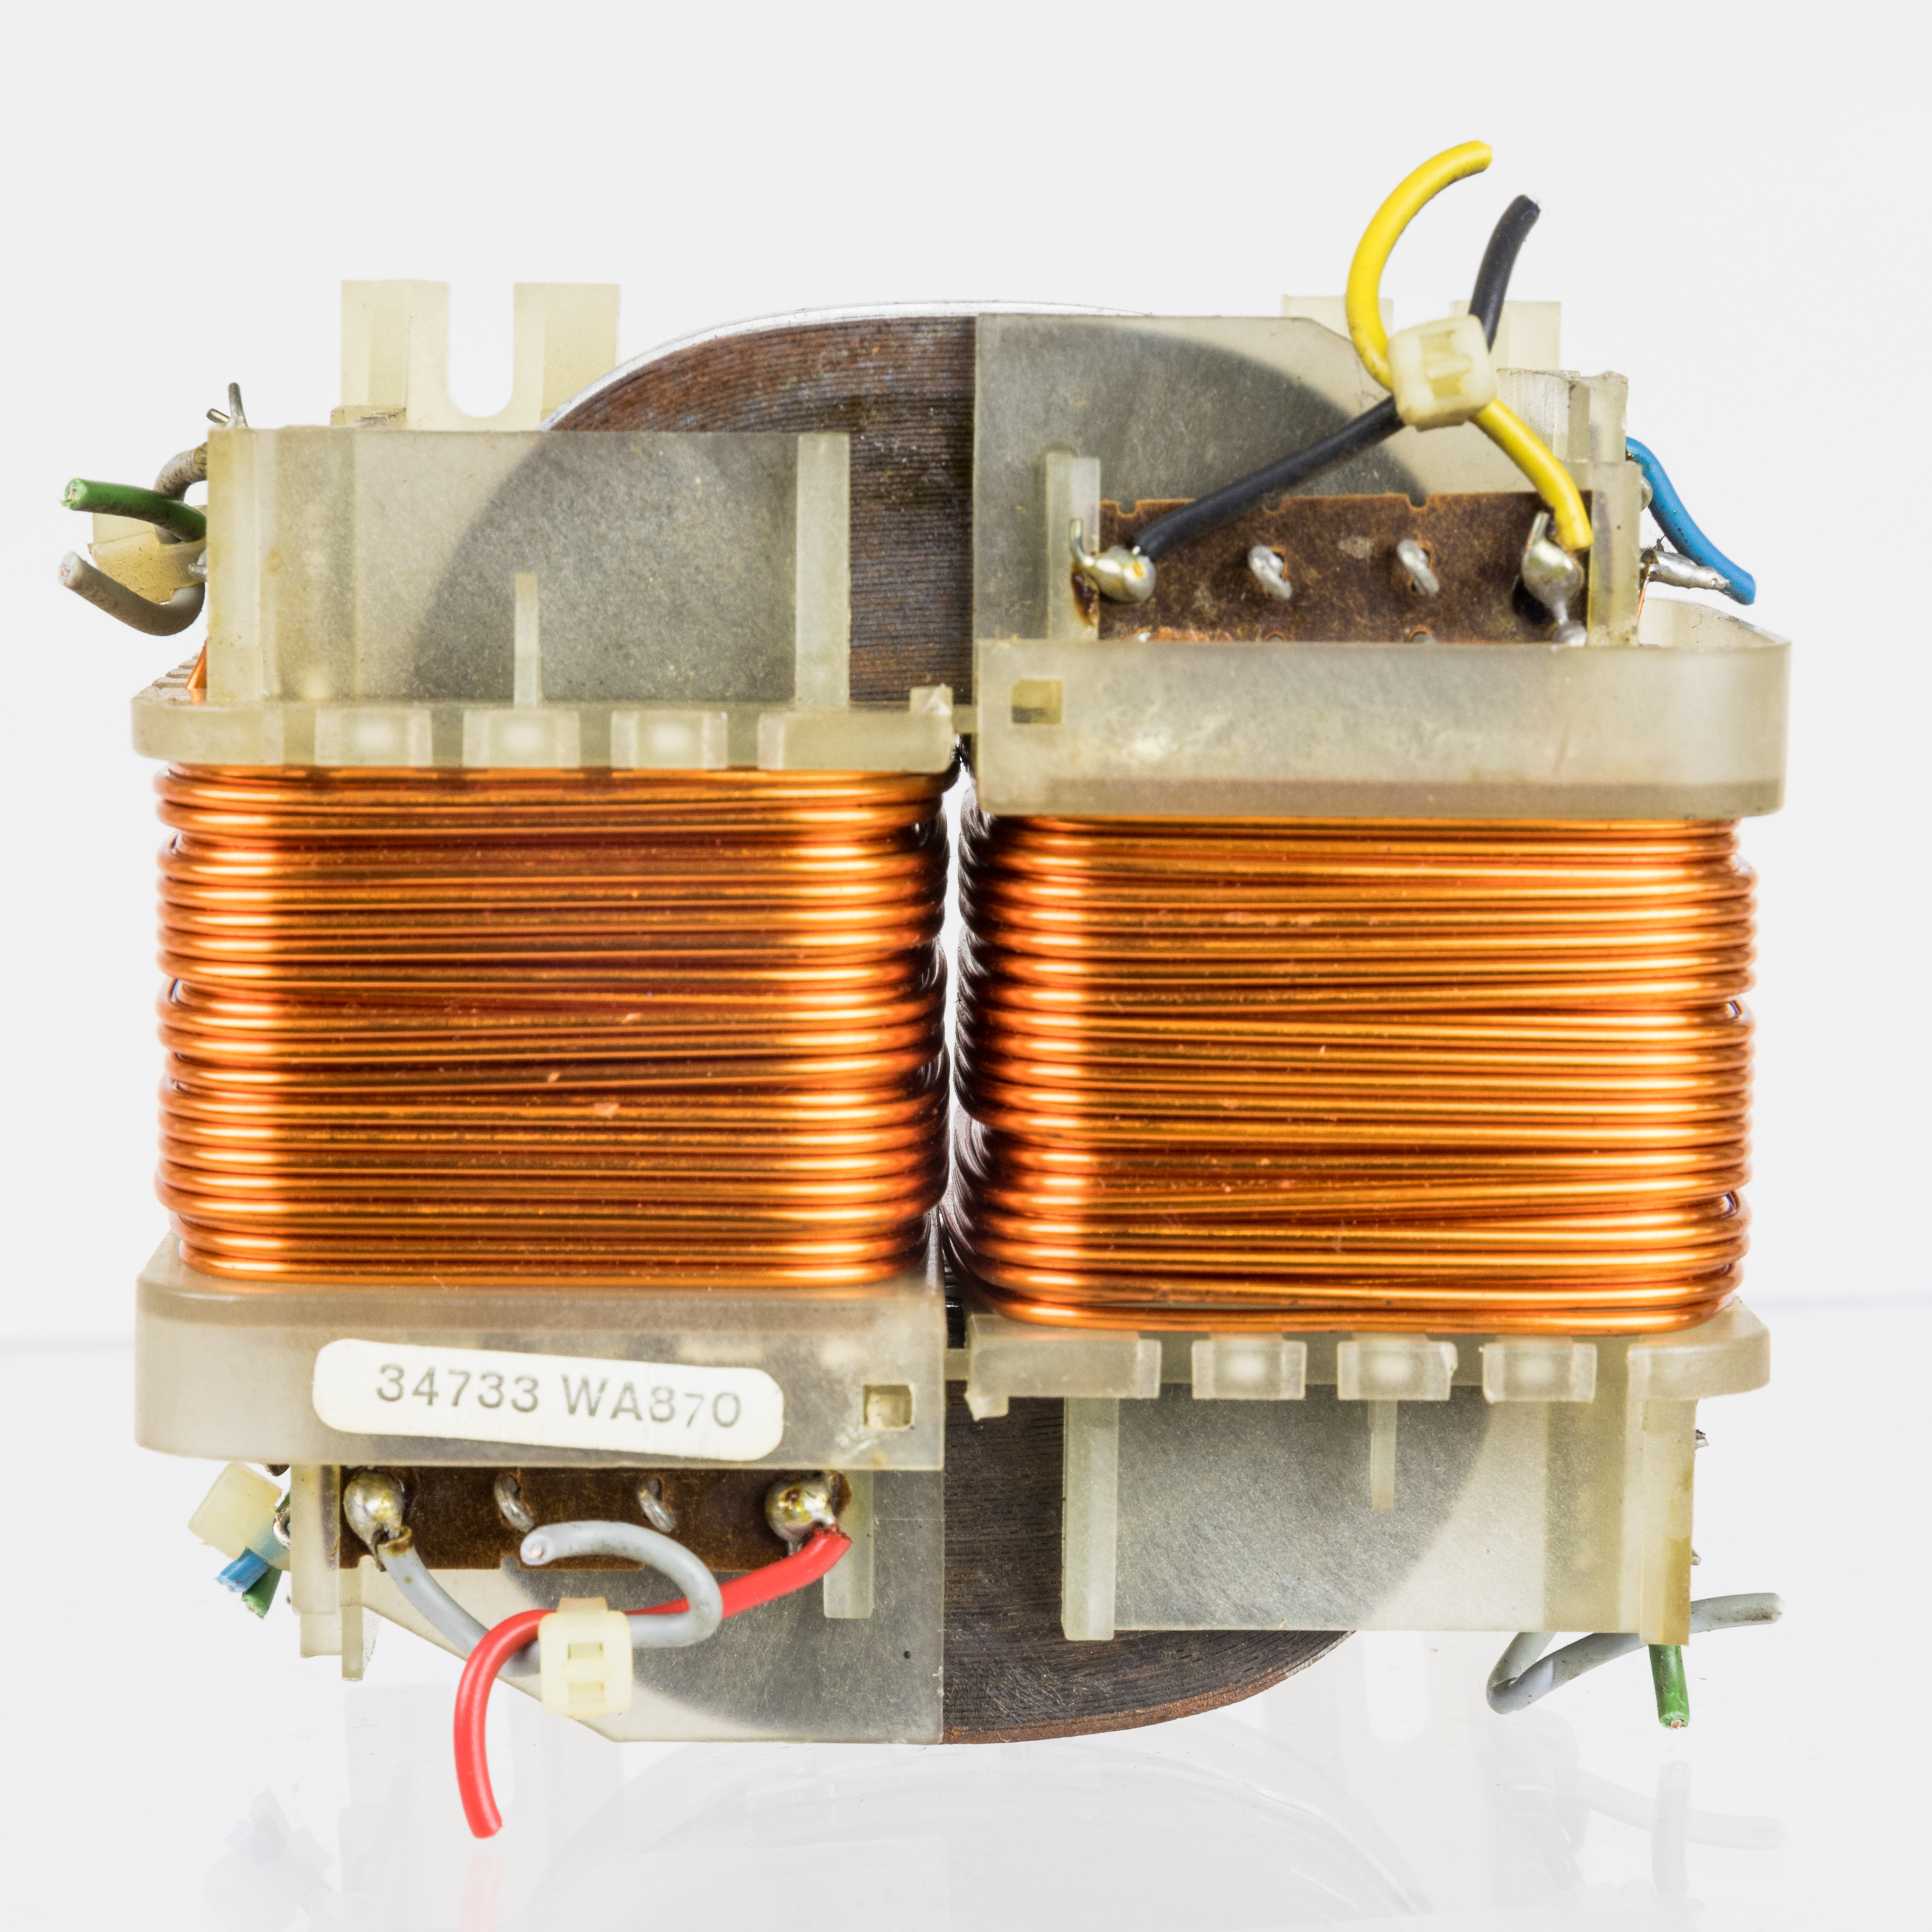
\includegraphics[height=0.7\textwidth]{transformer.jpg}
            \end{center}
            \caption{Bild eines Transformators mit Eisenkern\cite{wiki_transformer}}
        \end{figure}

    \end{columns}
\end{frame}

\subsection{Eigenschaften und Funktionsweise eines Transformators}
\begin{frame}
    \makeframetitle
    \begin{itemize}
        \item Wird nahezu überall verwendet
        \item Erlaubt die \textit{Umwandlung von Spannungen}
        \item Funktioniert \alert{ausschließlich} mit Wechselspannung
    \end{itemize}

    \begin{figure}
        \begin{center}
            \begin{circuitikz}
                \draw
                (0, 0) node[transformer core](T){};
            \end{circuitikz}
        \end{center}
        \caption{Schaltkreiszeichen eines Transformators mit Eisenkern}
    \end{figure}
\end{frame}

\begin{frame}
    \makeframetitle
    \begin{itemize}
        \item An der Primärspule liegt eine \textit{Wechsel}spannung $U_P$ an
        \item Die Primärspule \textit{induziert} eine Wechselspannung $U_S$ an
            der Sekundärspule
        \item Für einen \textit{idealen} und \textit{unbelasteten}
            Transformator gilt: \\
            $\frac{U_S}{U_P} = \frac{N_S}{N_P}$
    \end{itemize}
    \pause
    \begin{exampleblock}{Beispiel}
        geg.: $N_P = 5; N_S=10; U_P = 10V$
        \pause
        \begin{align}
            \frac{U_S}{U_P} &= \frac{N_S}{N_P} | \cdot U_P \\
            U_S &= \frac{N_S}{N_P} \cdot U_P \\ 
            \Rightarrow U_S &= \frac{10}{5} \cdot 10\unit\volt =
            \underline{20\unit\volt}
        \end{align}
    \end{exampleblock}
\end{frame}

\begin{frame}
\makeframetitle
\begin{figure}
    \begin{columns}
        \column{0.5\textwidth}
        \begin{center}
            \includegraphics[height=0.80\textheight]{trans_ani1.jpg}
        \end{center}
        \column{0.5\textwidth}
        \caption{LEIFIphysik Animation\cite{leifi_trans_ani1}}
    \end{columns}
\end{figure}
\end{frame}

\subsection{Weitere Verwendungen von Spulen}
\begin{frame}
    \makeframetitle
    \begin{columns}
        \column{0.6\textwidth}
        \begin{itemize}
            \item Elektromotoren
            \item Relais
            \item Lautsprecher
            \item Elektromagneten
            \item Stromflussglättung
            \item usw...
        \end{itemize}
        \column{0.4\textwidth}
        \begin{figure}
            \begin{center}
                \includegraphics[width=0.9\textwidth]{relais.jpg}
            \end{center}
            \caption{Bild eines Relais\cite{wiki_relais}}
        \end{figure}
        
    \end{columns}
\end{frame}


\nocite{*}
\section{Quellenverzeichnis}
\begin{frame}[allowframebreaks]
    \frametitle{Bilder und Illustrationen}
    \framesubtitle{Literatur}

    \printbibliography[nottype=online,heading=subbibliography, title={Informationsquellen}]
\end{frame}

\begin{frame}[allowframebreaks]
    \frametitle{Informationsquellen und Sachtexte}
    \framesubtitle{Literatur}
    \printbibliography[type=online, heading=subbibliography,title={Bilder und Illustrationen}]
\end{frame}

\end{document}
